\documentclass[nonatbib,numbers,10pt]{llncs}

% Font
%\usepackage[scaled]{helvet}
%\renewcommand\familydefault{\sfdefault} 
%\usepackage[T1]{fontenc}

\usepackage{fontspec}
%\setmainfont{Nimbus Sans L}
%\setmainfont{Phetsarath OT}
\setmainfont{Liberation Sans}
%\DeclareMathSizes{10}{8}{7}{6}

% Geometry
\usepackage{geometry}
\geometry{
	a4paper,
	total={170mm,257mm},
	top=4.5cm,
	right=4cm,
	bottom=6.5cm,
	left=5cm,
}

\usepackage{epigraph}
% Math
\usepackage{amsmath}
\usepackage{amssymb}
\usepackage{stmaryrd}
% Code listing
\usepackage{minted}
%\usemintedstyle{friendly}
\usemintedstyle{tango}
\usepackage{algorithm}
\usepackage[noend]{algpseudocode}
% Colors
\usepackage{xcolor}
\colorlet{CodeBg}{gray!90}
\usepackage{color, colortbl}
\definecolor{Gray}{rgb}{0.9,0.9,0.9}
\definecolor{bblue}{HTML}{1D577A}
\definecolor{rred}{HTML}{C03425}
\definecolor{ggreen}{HTML}{8BB523}
\definecolor{ppurple}{HTML}{6B1B7F}
\definecolor{pblack}{HTML}{000000}
\definecolor{pyellow}{HTML}{C0B225}
% Graphs
\usepackage{tikz}
\usetikzlibrary{calc}
\usetikzlibrary{trees}
\usetikzlibrary{positioning}
\usepackage{pgfplots}
% Graphics
\usepackage{graphics}
\graphicspath{{figures/}} % Location of the graphics files

\newcommand\todo[1]{\textcolor{red}{#1}}
\newcommand{\w}[1]{\textit{"#1"}}
\newcommand\s{\textsc}

\newcommand{\Order}[5]{
	\[
	\mathcal{#1}_{#5}\llbracket #2 \leftarrow #3 \mid \{ #4 \} \rrbracket.
	\]
}
\newcommand{\Orderr}[5]{
	\mathcal{#1}_{#5}\llbracket #2 \leftarrow #3 \mid \{ #4 \} \rrbracket.
}
\newcommand{\Ord}[4]{\Order{O}{#1}{#2}{#3}{#4}}
\newcommand{\Or}[4]{\Orderr{O}{#1}{#2}{#3}{#4}}
\newcommand{\Con}[4]{\Order{C}{#1}{#2}{#3}{#4}}

\title{$D^3$ as a 2-MCFL}
\author{}
\institute{}

\begin{document}
\maketitle

\begin{abstract}
We discuss the open problem of parsing the Dyck language of 3 symbols, $D^3$, using a 2-Multiple Context-Free Grammar. We tackle this problem by implementing a number of novel techniques and present the associated software packages we developed.
\end{abstract}

\keywords{Dyck Language; multiple context free grammars (MCFG)}


\section{Introduction}\label{sec1}
Our goal with this paper is the analysis of the 3-dimensional Dyck Language, $D^3$, under the scope of a 2-multiple context-free language, 2-MCFL. For brevity's sake, this chapter only serves as a brief introductory guide towards relevant papers, where the interested reader will find definitions, properties and various correspondences of the problem. 

$D^3$ is defined over a lexigraphically ordered alphabet ($a$, $b$, $c$) as the generalized language of well-balanced parentheses\cite{moortgat}. We attempt to model $D^3$ via a 2-MCFG; the class of multiple context free grammars that operate on pairs of strings\cite{gotzmann}.

There are a number of interesting correspondences to $D^3$. Firstly, a word of $D^3$ can be presented as a \textit{standard Young Tableau}, which is a rectangular table with strictly ascending rows/columns containing as entries the numbers $\{1,2,\dots,n\}$ where $n$ the  total number of symbols in the word. The Young Tableau can be obtained by placing (in order) each character's index to the row corresponding to its lexicographical ordering (e.g. an $a$ is placed on the first row)\cite{moortgat}. 

Another correspondence exists between $D^3$ and combinatorial \textit{Spider Webs}, a special category of directed planar graphs embedded on a disk\cite{petersen}. Spider Webs can be obtained through the application of a set of rules, known as the \textit{Growth Algorithm}, which operates on pairs of neighbouring nodes, collapsing them into a singular intermediate node, transforming them into a new pair or eliminating them altogether. At termination, this process produces a well-formed Spider Web, which, in the context of $D^3$, can be interpreted as a visual representation of parsing a word.

A bijection links Young Tableaux with Spider Webs. Specifically, the \textit{Jeu-de-taquin} algorithm can be applied on a Young Tableau, which transforms it to another one through an act called \textit{promotion}. Subsequent promotions will eventually result in the initial tableau. Promotion thus defines an equivalence class, which we call an \textit{orbit}\cite{petersen}.

\section{Modeling Techniques}\label{sec2}
We now present a number of novel techniques that we developed as an attempt to solve the problem at hand, incrementally moving towards more complex and abstract grammars. For the purpose of experimentation we have implemented these techniques, based on a software library for parsing MCFGs\cite{ljunglof}. 

\subsection{Triple Insertion}
To set things off, we start with the grammar of \textit{triple insertion}. This grammar operates on non-terminals $\s{W}(x,y)$, producing a $\s{W}(x',y')$ with an additional triplet \textit{a, b, c} that respects the partial orders $x<y$ and $a<b<c$. The end-word is produced through the concatenation of $(x,y)$.

\begin{figure}
  \begin{minipage}{0.45\textwidth}
  	\centering
    \begin{align}
	\setcounter{equation}{0}
	\s{S}(xy) \leftarrow \s{W}(x,y)&. \\
	\s{W}(\epsilon, xy\textbf{abc}) \leftarrow \s{W}(x,y)&. \\
	... \nonumber \\
	\setcounter{equation}{60}
	\s{W}(\textbf{abc}xy, \epsilon) \leftarrow \s{W}(x,y)&. \\
	\s{W}(\epsilon, \textbf{abc})&. \\
	... \nonumber \\
	\setcounter{equation}{64}
	\s{W}(\textbf{abc}, \epsilon)&.
	\end{align}
	\caption{Grammar of triple insertions}
    \label{fig:1}
  \end{minipage} \hspace{0.1\textwidth}
  \begin{minipage}{0.45\textwidth}
  	\centering
    \begin{align*}
    \setcounter{equation}{0}
	\s{C}^-(\epsilon, xyzw) \leftarrow \s{A}^+(x,y),\ \s{B}^+(z,w)&. \\
	\s{C}^-(x, xyzw) \leftarrow \s{A}^+(x,y),\ \s{B}^+(z,w)&. \\
	\s{C}^-(xy, zw) \leftarrow \s{A}^+(x,y),\ \s{B}^+(z,w)&. \\
	\s{C}^-(xyz, w) \leftarrow \s{A}^+(x,y),\ \s{B}^+(z,w)&. \\
	\s{C}^-(xyzw, \epsilon) \leftarrow \s{A}^+(x,y),\ \s{B}^+(z,w)&.
	\end{align*}
	\caption{Interaction between $\s{A}^+$ and $\s{B}^+$}
	\label{fig:interaction}
  \end{minipage}
\end{figure}


Despite being conceptually simple, this grammar consists of a large number of rules. Its expressivity is also limited; the prominent weak point is its inability to manage the effect of \textit{straddling}, namely the generation of words whose substituents display complex interleaving patterns.
\subsection{Adding States: Meta-Grammars}
To counteract the limited performance of the above grammar, we introduce more states to describe incomplete words; that is, words that either have an extra symbol or miss one. The former are positive states, whereas the latter are negative. The addition of these extra states would allow for more intricate interactions. For instance, a state $\s{A}^{+}$ could interact with a $\s{B}^{+}$ to produce a $\s{C}^{-}$ in a multitude of different ways. Interestingly, there is a direct correspondence between these states and the nodes of Petersen's growth algorithm.

These new emerging interactions vastly increase the amount of rules that need to be considered. Moreover, for each pair interaction, different constraints pertaining to the order of the permuted concatenated strings need to be preserved. This necessitates a more abstract view of the grammar as whole. To that end, we define $\mathcal{O}$ as the \textit{meta-rule} which, given a rule format, a set of partial orders (over the tuple indices of its premises and/or newly added terminal symbols), and the MCFG dimensionality, automatically generates all the order-respecting permutations. We thereby reduce the manual labour required to transcribe and debug individual rules.
\Ord{\s{C}^-}{\s{A}^+, \s{B}^+}{t_{11} < t_{12} < t_{21} < t_{22}}{2}
As an example, we give the above meta-rule which demonstrates the interaction between $\s{A}^+$ and $\s{B}^+$ to produce a new $\s{C}^-$ state, as depicted in Fig.\ref{fig:interaction}.

This additional abstraction, however, is not enough on its own. We still needed the ability to enforce additional constraints related not to the order, but rather the positions of concatenated strings. To make this clear, let us present the unique case of $B^{-}$. Unlike other negative states, $B^{-}(t_{11},\ t_{12})$ has no direct closure unless we actually know it to contain its extra $a$ in the left-side string $t_{11}$ and its extra $c$ in $t_{12}$ (we refer to this distinction between a position-blind and a position-aware state as \textit{refinement}). In that case alone are we allowed to insert the missing $b$ (e.g. as obtained from a $B^{+}(t_{21},\ t_{22})$ between $t_{11}$ and $t_{12}$. But in order to automatically generate $B^{-}$ states for which this additional condition holds, we need to keep note of the origin of the extra $a$ and $c$, and filter out the rules generated by $\mathcal{O}$ accordingly. We thus define $\mathcal{C}$ as a stricter version of $\mathcal{O}$, which constraints the rules according to the positions the premise tuples may occupy (after concatenation) in the conclusion's tuple.
\Con{\textsc{B}^-}{\textsc{A}^+, \textsc{C}^+}{t_{11}^l < t_{12}^l,\ t_{21}^r < t_{22}^r}{2}
In the above notation, we illustrate that $\textsc{B}^{-}$ may be constructed from $\textsc{A}^{+}(t_{11},\ t_{12})$ and $\textsc{C}^{+}(t_{21},\ t_{22})$ only as long as the partial orders $(t_{11},\ t_{12})$ and $(t_{21},\ t_{22})$ are independently satisfied and $t_{11}$, $t_{12}$ are both placed on the left element of the new state's tuples, while $t_{21}$ and $t_{22}$ on the right. This of course only allows for $\textsc{C}^{-}$ to consist of the tuple $(t_{11}t_{12},\ t_{21}t_{22})$.

The above abstractions significantly accelarated the process of creating and testing grammars, as they allowed us to simply describe rules instead of explicitly defining them. We thus moved from the lower level of grammars to the higher level of \textit{meta-grammars}, or grammars of grammars. This strikes a resemblance to the notion of \textit{declarative programming}, where one only cares about what needs to be computed, rather than how.

\subsection{Refining States: Rule Inference}\label{aris}	
Perhaps expectedly, the improved performance of our new approach again proved insufficient to completely parse $D^3$. New problems started arising when trying to solve longer words; even though they were sound, our rules failed to make full use of the expressivity that a 2-MCFG allows. We soon realized that we have over-constrained our rules by making them comply to the worst-case scenario. Following the example of Fig.~\ref{fig:interaction}, if we had kept memory of the position of $a$ in a \textit{refined} version of  $A^{+}(x,y)$, we could allow new rules to exist, such as \[\s{C}^-(xz,wy) \leftarrow \s{A}^+_{left}(x,y),\ \s{B}^+(z,w).\] in the case of the extra $a$ residing in $x$. Splitting each state into multiple different, refined states that now provide knowledge of their extra characters' positions, we could model vastly more interactions.

At this point, the abstraction offered by our meta-grammars did not cover our needs anymore. The same difficulty that we had encountered before was prominent once more, except now at an even higher level. Transcribing meta-rules and proofreading them was time consuming and error-prone, effectively hindering our progress. In order to test a new hypothesis pertaining to the refined states we would again have to go through a lot of arid work.

As a solution to the aforementioned limitations, we designed a system that can automatically create a full-blown m-MCFG given only the states it consists of. To accomplish this, we assign each state a unique \textit{descriptor} that specifies (up to an extent) the content of its tuple's elements. Aligning these descriptors with the tuple, we can then infer the descriptor of the resulting tuple of every possible state interaction. For the subset of thοse interactions whose resulting descriptor is matched with a state, we can now automatically infer the rule.

Formally, the system is initialized with a map $\mathcal{D}$, whose domain, $dom(\mathcal{D})$, is a set of \textit{state identifiers} and its codomain, $codom(\mathcal{D})$, is the set of their corresponding \textit{state descriptors}.

\begin{algorithm}
\caption{ARIS: Automatic Rule Inference System}\label{euclid}
\begin{algorithmic}
\Procedure{aris}{$\mathcal{D}$}
	\For{$X \in dom(\mathcal{D})$}
		\State $(d_1,\dots ,d_n) \leftarrow \mathcal{D}(X)$
		\State \textbf{yield} $X(d_1,\dots,d_n).$
	\EndFor
	\For{$x,Y \in dom(\mathcal{D})^2$}
		\State $X_{ord} \leftarrow t_{11}<\dots<t_{1n}$ 
		\State $Y_{ord} \leftarrow t_{21}<\dots<t_{2n}$ 
		\State $new\_order \leftarrow \Or{\_}{X,Y}{X_{ord}, Y_{ord}}{2}$
		\For{$(d_1,...,d_n) \in new\_order$}
			\For{$S' \in \textsc{eliminate}((d_1,\dots ,d_n), \mathcal{D})$}
				\State \textbf{yield} $S'(d_1,\dots ,d_n) \leftarrow X, Y.$
			\EndFor
		\EndFor
	\EndFor
\EndProcedure
\\
\Procedure{eliminate}{$(d_1,\dots ,d_n), \mathcal{D}$}
	\For{$matches \in \textsc{match\_all}(t_1, ..., t_n)$}
		\For{$i \in 0\dots n/3$}
			\For{$S' \in \textsc{remove\_all}(matches, i)$}
				\If {$S' \in codom(\mathcal{D})$}
					\State \textbf{yield} $S'$
				\EndIf				
			\EndFor
		\EndFor
	\EndFor
\EndProcedure
\\
\Procedure{match\_all}{$t_1,...,t_n$}
	\State \textbf{return} \textit{all possible ways to match a,b,c triplets}
\EndProcedure
\\
\Procedure{remove\_all}{$matches, i$}
	\State \textbf{return} \textit{all possible ways to annihilate i matches}
\EndProcedure
\end{algorithmic}
\end{algorithm}

Note that the above algorithm can easily be generalized to be applicable to the combination of an arbitrary number of states, but doing so would render it computationally infeasible. By using \textit{ARIS}, one needs only specify a grammar's states and its descriptors, thus eliminating the need to explicitly define rules or even meta-rules.

\section{Implementation}\label{sec3}
Enabled by the machinery described in the previous chapter we performed a multitude of tests using different grammars. In this chapter we describe a few of these grammars that we deem as milestones of our progression, in ascending order of complexity. We also present some statistics to allow for a direct comparison to be made between them. For the purposes of this project we use a version of MCFParser \cite{ljunglof} as our backend, which we adapted to our needs\footnote{The original can be found at https://github.com/heatherleaf/MCFParser.py}.
\subsection{Grammars}
In the grammars below, when applying meta-rules, we consider $t_{ij}$ to be the j-th tuple element of the i-th input state.
\paragraph{G$_0$: Triple insertion}
This very simple grammar consists of simply the rules of triple-insertion on a single non-terminal state $\s{W}(x,y)$, as described in chapter 2. Using the $\mathcal{O}$ abstraction, this grammar can be simply expressed as:
\begin{align*}
&\s{S}(xy) \leftarrow \s{W}(x,y). \\
&\Or{\s{W}}{\epsilon}{a < b < c}{2} \\
&\Or{\s{W}}{\s{W}}{t_{11} < t_{12},\ a < b < c}{2}
\end{align*}
\paragraph{G$_1$: Interleaving words}
Benefiting from the added expressivity of $\mathcal{O}$, we can extend the previous grammar with a single meta-rule that allows two non-terminals $W(x,y)$, $W(z,w)$ to interact with one another, producing rearranged tuple concatenations and allowing some degree of straddling to be generated.
\vspace{-\topsep}
\begin{align*}
& \quad\quad\quad\quad \vdots \\
&\Or{\s{W}}{\s{W}, \s{W}}{t_{11} < t_{12},\ t_{21} < t_{22}}{2}
\end{align*}
\paragraph{G$_2$: Incomplete words}
This grammar largely expands upon the concept of state interaction of the previous grammar, replacing the idea of triple insertion with the use of non-terminals that correspond to types of incomplete words. There is a very clear and direct correspondence between this grammar and the non-swapping rules of the growth algorithm.
\begin{align*}
&\s{S}(xy) \leftarrow \s{W}(x,y). \\
&\Or{\s{W}}{\epsilon}{a < b < c}{2} \\
&\Or{\s{A}^+}{\epsilon}{a}{2} \\
&\Or{\s{B}^+}{\epsilon}{b}{2} \\
&\Or{\s{C}^+}{\epsilon}{c}{2} \\
&\Or{\s{A}^-}{\epsilon}{b < c}{2} \\
&\Or{\s{B}^-}{\epsilon}{a < c}{2} \\
&\Or{\s{C}^-}{\epsilon}{a < b}{2} \\
&\forall \ \s{K} \in \mathcal{S} \setminus \s{W}:\\ 
&\quad\quad\Or{\s{K}}{\s{K}, \s{W}}{t_{11} < t_{12},\ t_{21} < t_{22}}{2}
\end{align*}
Where $\mathcal{S}$ the set of states defined within this grammar:
\[
\mathcal{S}= \{\textsc{W},\ \textsc{A}^{+/-},\ \textsc{B}^{+/-},\ \textsc{C}^{+/-}\}
\]
\paragraph{G$_3$: Universal triple insertion}
Surprisingly, cases manageable by triple insertion could not be solved by the last grammar despite its elegance. After some thought, we realized that triple insertion is unique in the sense that it can insert three different terminals each at a different position, something that no other pair interaction can directly accomplish. We thus allowed triple insertion back into our last grammar, now at the level of each new state. To achieve this, we added the following universally quantified meta-rule:
\begin{align*}
& \quad\quad\quad\quad \vdots \\
&\forall \ \s{K} \in \mathcal{S} \setminus \s{W}:\\ 
&\quad\quad\Or{\s{K}}{\s{K}}{t_{11} < t_{12},\ a < b < c}{2}
\end{align*}
\paragraph{G$_4$: Refined non-terminals}
As the peak of our efforts, we replace non-terminals with their refined versions as presented in section \ref{aris}. $A^{+}(x,y)$ is now split into $A^{+}_{left}(x,y)$ and $A^{+}_{right}(x,y)$, with the extra $a$ residing in $x$ and $y$ in each case respectively. To generate this grammar, we use ARIS initialized with the following $\mathcal{D}$ map:

\begin{minipage}{.2\textwidth}
\begin{align*}
\s{W} &\mapsto (\epsilon, \epsilon) \\
\s{A}^+_{l} &\mapsto (a, \epsilon) \\
\s{A}^+_{r} &\mapsto (\epsilon, a) \\
\s{B}^+_{l} &\mapsto (b, \epsilon) \\
\s{B}^+_{r} &\mapsto (\epsilon, b) \\
\s{C}^+_{l} &\mapsto (c, \epsilon) \\
\s{C}^+_{r} &\mapsto (\epsilon, c) \\
\s{A}^-_{l} &\mapsto (bc, \epsilon) 
\end{align*}
\end{minipage}
\begin{minipage}{.2\textwidth}
\begin{align*}
\s{A}^-_{r} &\mapsto (\epsilon, bc) \\
\s{A}^-_{l, r} &\mapsto (b, c) \\
\s{B}^-_{l} &\mapsto (ac, \epsilon) \\
\s{B}^-_{r} &\mapsto (\epsilon, ac) \\
\s{B}^-_{l, r} &\mapsto (a, c) \\
\s{C}^-_{l} &\mapsto (ab, \epsilon) \\
\s{C}^-_{r} &\mapsto (\epsilon, ab) \\
\s{C}^-_{l, r} &\mapsto (a, b)
\end{align*}
\end{minipage}
\subsection{Results}
We display three charts, depicting the number of rules, percentage of counter-examples and computation times of each of our grammars for $D^3_n$ with $n$ ranging from $2$ to $6$. The charts reveal two obvious trends; as grammars get more complex, the number of failing parses steadily declines. This however comes at the cost of rule size growth, which in turn is associated with dramatically exploding computation times. What this practically means is that we are unable to continue testing more elaborate grammars or scale our results to higher orders of $n$ (recall that $| \! | D^3_n | \! |$ also has a very rapid rate of expansion).
\begin{figure}[h!]
% Rule size
\hspace*{-.5cm}
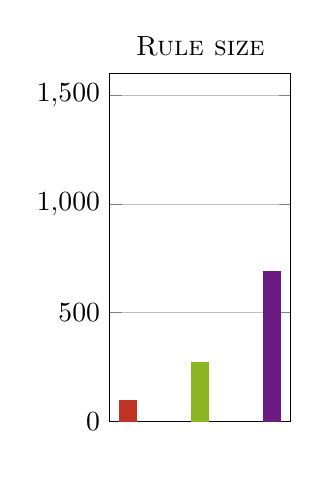
\begin{tikzpicture}
    \begin{axis}[
        width  = 0.32*\textwidth,
        height = 6cm,
        major x tick style = transparent,
        ybar=20,
        bar width=6pt,
        ymajorgrids = true,
        ylabel = {\textsc{Rule size}},
        every axis x label/.style={
  			  at={(ticklabel* cs:1.05)},
  			  anchor=west,
  			  },
			every axis y label/.style={at={(current axis.north)},above=1mm},
        symbolic x coords={$ $},
        xtick = data,
        scaled y ticks = false,
        enlarge x limits=0,
        ymin=0,
        legend cell align=left,
        legend style={
        		at={(0.5,-0.15)},
				anchor=north,
				legend columns=-1
			},
    ]
        \addplot[style={bblue,fill=bblue,mark=none}]
            coordinates {($ $, 65)};
        \addplot[style={rred,fill=rred,mark=none}]
             coordinates {($ $,95)};
        \addplot[style={ggreen,fill=ggreen,mark=none}]
             coordinates {($ $,270)};
        \addplot[style={ppurple,fill=ppurple,mark=none}]
             coordinates {($ $,690)};
        \addplot[style={pyellow,fill=pyellow,mark=none}]
             coordinates {($ $,1456)};
    \end{axis}
\end{tikzpicture}
% Counter-examples
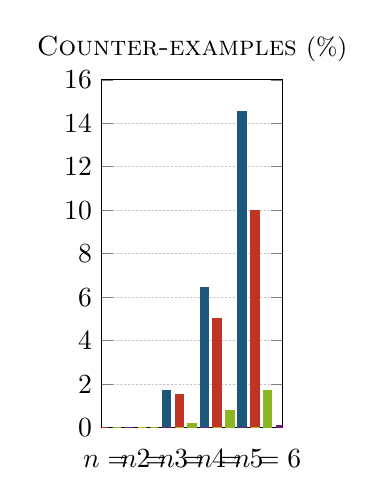
\begin{tikzpicture}
    \begin{axis}[
        width  = 0.32*\textwidth,
        height = 6cm,
        major x tick style = transparent,
        ybar=4*\pgflinewidth,
        bar width=3pt,
        ymajorgrids = true,
        ylabel = {\textsc{Counter-examples} \small (\%)},
        every axis x label/.style={
  			  at={(ticklabel* cs:1.05)},
  			  anchor=west,
  			  },
			every axis y label/.style={at={(current axis.north)},above=1mm},
        symbolic x coords={$n=2$,$n=3$,$n=4$,$n=5$,$n=6$},
        xtick = data,
        scaled y ticks = false,
        enlarge x limits=0.1,
        ymin=0,
        legend cell align=left,
        legend style={
        		at={(0.5,-0.15)},
				anchor=north,
				legend columns=-1
			},
		ytick={0, 2, ..., 17},
		y grid style={densely dotted, line cap=round},
    ]
        \addplot[style={bblue,fill=bblue,mark=none}]
            coordinates {($n=2$, 0) ($n=3$,0) ($n=4$,1.7) ($n=5$,6.42) ($n=6$,14.55)};
        \addplot[style={rred,fill=rred,mark=none}]
             coordinates {($n=2$,0) ($n=3$,0) ($n=4$,1.5) ($n=5$,5) ($n=6$,10)};
        \addplot[style={ggreen,fill=ggreen,mark=none}]
             coordinates {($n=2$,0) ($n=3$,0) ($n=4$,0.2) ($n=5$,0.8) ($n=6$,1.7)};
        \addplot[style={ppurple,fill=ppurple,mark=none}]
             coordinates {($n=2$,0) ($n=3$,0) ($n=4$,0) ($n=5$,0) ($n=6$,0.1)};
        \addplot[style={pyellow,fill=pyellow,mark=none}]
             coordinates {($n=2$,0) ($n=3$,0) ($n=4$,0) ($n=5$,0) ($n=6$,0.05)};

    \end{axis}
\end{tikzpicture}
% Computation Time
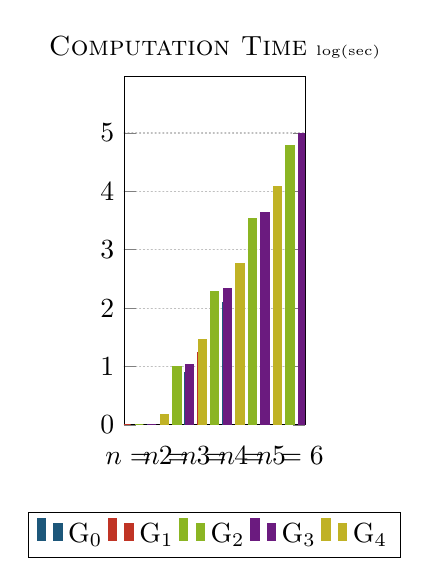
\begin{tikzpicture}
    \begin{axis}[
        width  = 0.32*\textwidth,
        height = 6cm,
        major x tick style = transparent,
        ybar=4*\pgflinewidth,
        bar width=3pt,
        ymajorgrids = true,
        ylabel = {\textsc{Computation Time} \tiny log(sec)},
        every axis x label/.style={
  			  at={(ticklabel* cs:1.05)},
  			  anchor=west,
  			  },
			every axis y label/.style={at={(current axis.north)},above=1mm},
        symbolic x coords={$n=2$,$n=3$,$n=4$,$n=5$,$n=6$},
        xtick = data,
        scaled y ticks = false,
        enlarge x limits=0.1,
        ymin=0,
        legend cell align=left,
        legend style={
        		at={(0.5,-0.25)},
				anchor=north,
				legend columns=-1
			},
		ytick={0, 1, ..., 5},
		y grid style={densely dotted, line cap=round},
    ]
		 \addplot[style={bblue,fill=bblue,mark=none}]
           coordinates {($n=2$, 0) ($n=3$,-0.3) ($n=4$,0.9) ($n=5$,2.1) ($n=6$,3.37)};           
        \addplot[style={rred,fill=rred,mark=none}]
             coordinates {($n=2$,0) ($n=3$,0) ($n=4$,1.23) ($n=5$,2.39) ($n=6$,3.73)};             
        \addplot[style={ggreen,fill=ggreen,mark=none}]
             coordinates {($n=2$,0) ($n=3$,1) ($n=4$,2.28) ($n=5$,3.54) ($n=6$,4.79)};
        \addplot[style={ppurple,fill=ppurple,mark=none}]
             coordinates {($n=2$,0) ($n=3$,1.04) ($n=4$,2.34) ($n=5$,3.64) ($n=6$,4.99)};
        \addplot[style={pyellow,fill=pyellow,mark=none}]
             coordinates {($n=2$,0.17) ($n=3$,1.46) ($n=4$,2.77) ($n=5$,4.09) ($n=6$,5.42)};
        \legend{G$_0$,G$_1$,G$_2$,G$_3$,G$_4$,G$_5$}
    \end{axis}
\end{tikzpicture}
\\
\caption{Performance measures}
\end{figure}

\section{Road to completeness}\label{sec4}
As the above results suggest, despite our best efforts the problem is yet unsolved. In this chapter we present a collection of unexplored ideas which we consider noteworthy. These ideas are related to the concept of formally concluding the completeness of a grammar, bypassing the computational problem of parsing through words in search of an example the tested grammar fails to generate.

\subsection{First-match policy and Relinking}
Possibly the most intuitive way of checking whether a word $w$ is part of $D^3_n$ is checking whether a pair of links occur that match $a_i$ to $b_i$ and $b_i$ to $c_i \ \forall i \in n$, where $x_i$ the i-th occurrence of symbol $x$ in $w$. We call this process of matching the \textit{first-match policy}.

\begin{figure}[h!]
\centering

\begin{tikzpicture}[every node/.style={anchor=base},xscale=.25,yscale=.4]
\node (n0) at (0,0) {$a$};
\node (n1) at (1,0) {$b$};
\node (n2) at (2,0) {$a$};
\node (n3) at (3,0) {$b$};
\node (n4) at (4,0) {$a$};
\node (n5) at (5,0) {$c$};
\node (n6) at (6,0) {$b$};
\node (n7) at (7,0) {$c$};
\node (n8) at (8,0) {$a$};
\node (n9) at (9,0) {$b$};
\node (n10) at (10,0) {$c$};
\node (n11) at (11,0) {$c$};
\draw (n0) edge [rred, bend left=90] (n1);
\draw (n1) edge [rred, bend right=90] (n5);
\draw (n2) edge [ggreen, bend left=90] (n3);
\draw (n3) edge [ggreen, bend right=90] (n7);
\draw (n4) edge [bblue, bend left=90] (n6);
\draw (n6) edge [bblue, bend right=90] (n10);
\draw (n8) edge [pyellow, bend left=90] (n9);
\draw (n9) edge [pyellow, bend right=90] (n11);
\end{tikzpicture}
\caption{First-match policy for \w{ababacbcabcc}}
\end{figure}

The question arises whether a grammar can accomplish inserting a triplet of $a$, $b$, $c$ in such a way that the triplet inserted always corresponds to a triplet matched by the first-match policy. If that were the case, it would be relatively easy to generalize this ability by induction to every $n \in \mathbb{N}$. Unfortunately, the answer is seemingly negative; the expressiveness provided by a 2-MCFG does not allow for the rather arbitrary insertions required. On a related note, being able to produce a word state $W(x,y)$ where $w=xy$ and $x$ any possible prefix of $w$ (i.e. all different comma positions $i$ for $i \in 0,1...3n$, gives no guarantee of being able to produce the same word with an extra triplet inserted due to the straddling property.

However, if rules existed that would allow for match-making and breaking, i.e. match \textit{relinking}, an inserted symbol could be temporarily matched with what might be its first match-policy in a local scope, and then relink it to its correct match when merging two words together. This might be an interesting prospect to look into.
\subsection{Growth Rules}
The growth rules presented in section~\ref{fig:rules} are formally sound and complete. Part of them also have a very straightforward correspondence with some of our rules. For the other part, namely the growth rules which produce two edges, there is no direct way of translating them into a 2-MCFG. Adding memory to the grammar by adding states that describe two neighbouring edges might seem appealing but would not solve the problem; two neighbouring edges can in turn interact with their next neighbours in a recursive fashion, which can not be accommodated by our current tuple representation. We cannot, however, rule out the possibility of the growth rules being scalably translatable into m-MCFG rules. In fact, such a translation would be a guarantee of completeness.
\subsection{Insights from promotion}
The act of promotion translates to cyclic rotation of the $A_2$ web \cite{petersen}. Perhaps an interesting question here is whether promotion can be handled by a 2-MCFG (as a \textit{context-free rewriting system}). If that is the case, it could be worth looking into the properties of orbits, to test for instance if there are promotions within an orbit that can be easier to solve than others. Solving a single promotion and transducing the solution to all other words belonging to the same orbit could then be a guideline towards completeness. The scale of such a task would of course be much greater, but the combination of these theoretical backbones into a unified body, combined with our mostly applied approach, could shed some light on the problem at hand.

\section{Tools}\label{tools}
\subsection{Grammar utilities}
We have implemented the modelling techniques we described in section \ref{sec2} and distributed a Python package, called \textbf{dyck}, which essentially provides the programmer with a \textit{domain-specific language} very close to this paper's mathematical notation. The following example demonstrates the similariry with G$_1$, defined in section \ref{sec3}:
\begin{minted}[baselinestretch=1.1, fontsize=\small]{python}
from dyck import *
G_1 = Grammar([
    ('S <- W', {(x, y)}),
    O('W', {(a, b, c)}),
    O('W <- W', {(x, y), (a, b, c)}),
    O('W <- W, W', {(x, y), (z, w)}),
])
\end{minted}

It ships with several examples, showcasing meta-grammars and \textsc{ARIS}, as well as the complete set of implemented grammars defined in section \ref{sec3}. The package provides a lot of features, relevant to experimentation on m-MCFGs, such as:
\begin{itemize}
\item Grammar selection
\item Time measurements
\item Rule/parse pretty-printing
\item Dyck-specific utilities
	\begin{itemize}
	\item Word generation
	\item Soundness/completeness checking
	\end{itemize}
\item Grammar (de)serialization
\end{itemize}

\subsection{Visualization}
As counter-examples began to grow in size and number, we realised the necessity of a visualization tool to mitigate the challenging task of identifying certain properties they exhibit.

To that end, we distribute another Python package, called \textbf{dyckviz}, providing a command-line tool, which allows the simultaneous visualization of tableau-promotion and web-rotation (grouped in their corresponding equivalence classes).

Young tableaux in an orbit are colored via the first-match-policy, which sheds some light on how the \textit{jeu-de-taquin} actually influences the structure of the correponding Dyck words. Interesting patterns have began to emerge, which still remain to be properly investigated.

Webs in a certain orbit, on the other hand, are rendered in a single PDF file (one web per page). Note that we represent them in a slightly simplified way compared to their definition in section \ref{sec2}, ignoring intermediate graph nodes that do not have corresponding non-terminals, as shown below:
\medskip
\begin{figure}[h!]
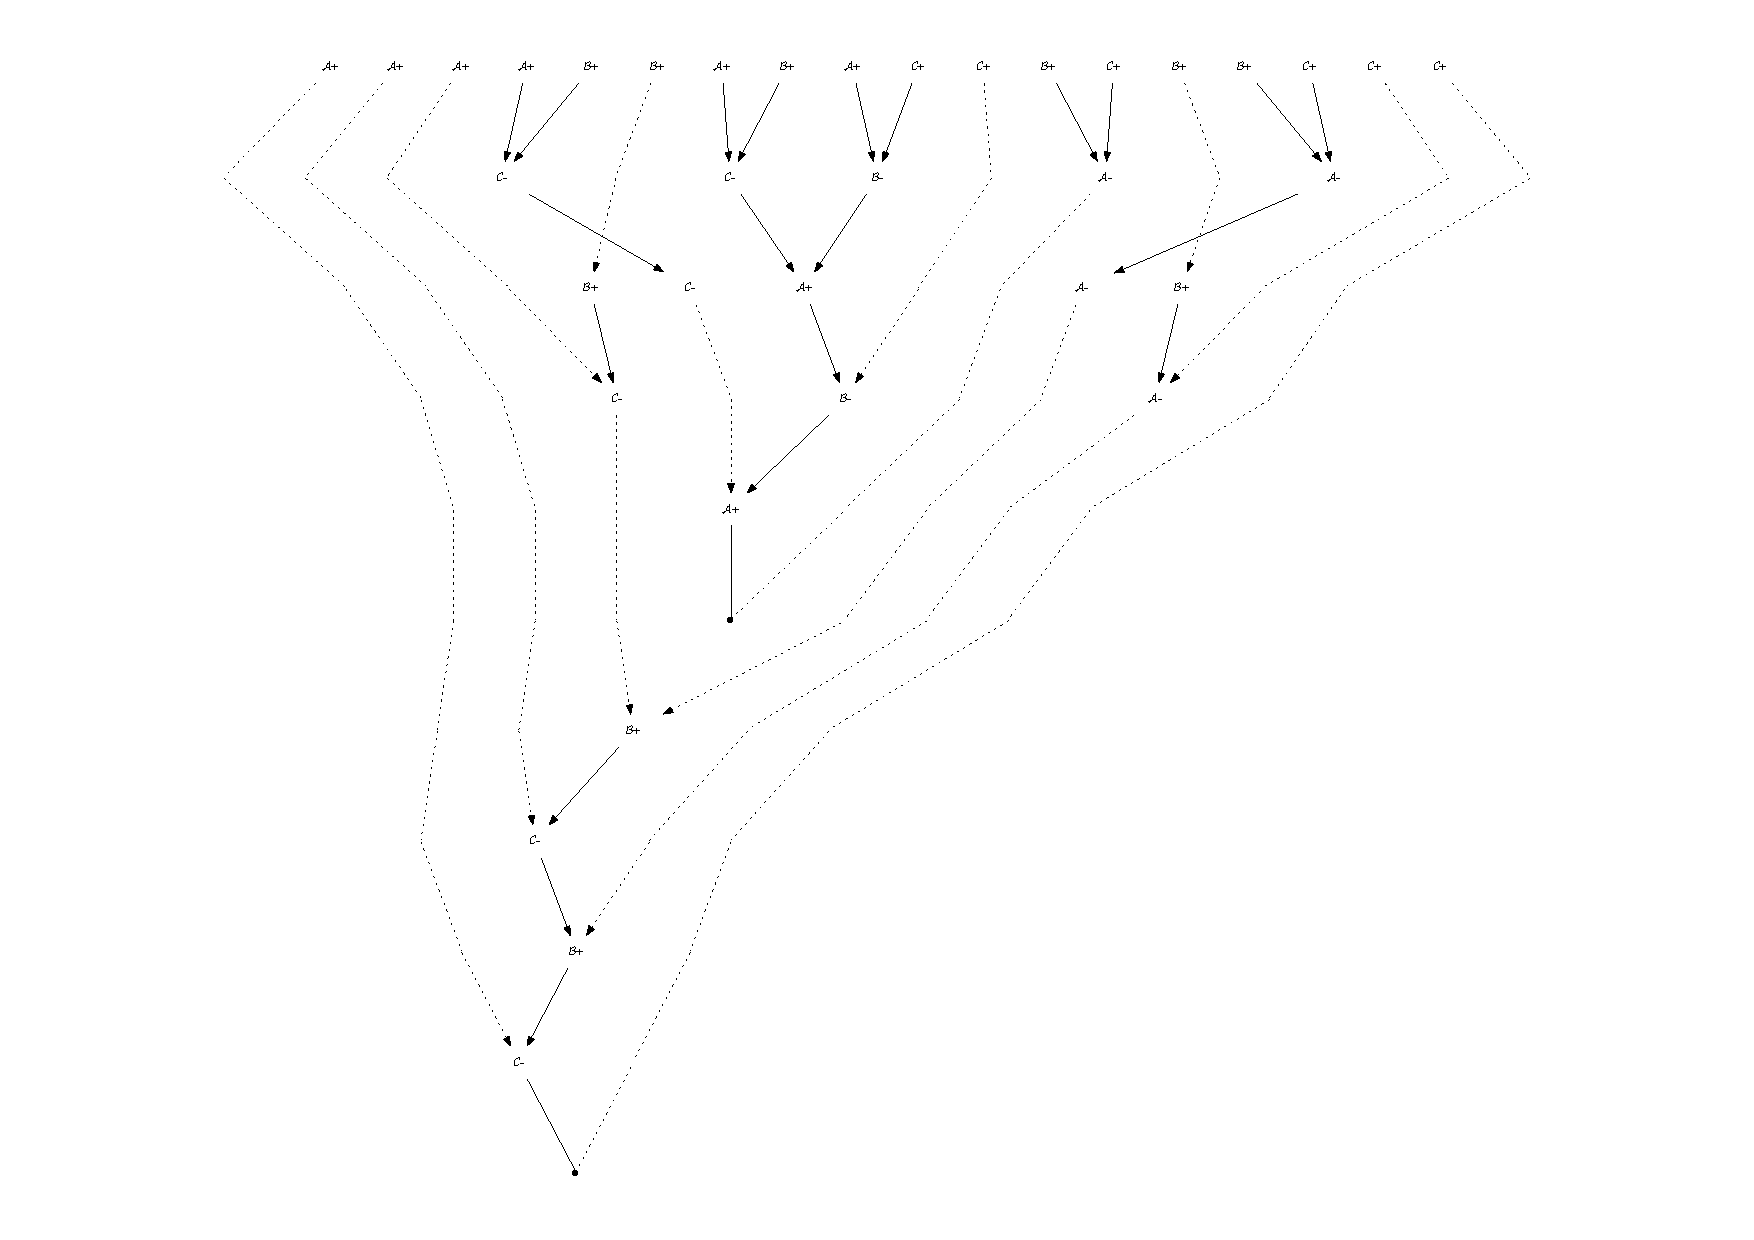
\includegraphics[width=1.05\columnwidth]{web.pdf}
\caption{Spider web of \w{abaacbbacbabaccbcc}}
\end{figure}

\section{Conclusion}
We tried to accurately present the intricacies of $D^3$ and the difficulties that arise when attempting to model it under the scope of a 2-MCFL. We have developed and introduced some interesting techniques and tools, which we believe can be of use even outside the problem's narrow domain. We have largely expanded on the existing tool suite available through the MCFParser and made it easier for it to accommodate MIX-style languages and systems of meta-grammars in general. 

Despite our best efforts, the question of whether $D^3$ can actually be encapsulated within a 2-MCFG still remains unanswered. Regardless, this problem has been very rewarding to pursue, and we hope to have intrigued the interested reader enough to further research the subject, use our code, or strive for a solution on his/her own.

\section*{Acknowledgements}
We would like to thank Dr. Michael Moortgat for introducing us to the problem and getting us started with valuable bibliography and some initial code.

%\newpage

\bibliographystyle{splncs03}
\bibliography{sources}

\end{document}
